%!TEX root = ../Thesis.tex
% Chapter Template

\chapter{Theory} % Main chapter title
\label{Theory} % Change X to a consecutive number; for referencing this chapter elsewhere, use \ref{ChapterX}
\lhead{Chapter \ref{Theory}. \emph{Theory}} % Change X to a consecutive number; this is for the header on each page - perhaps a shortened title

In this chapter the thesis will introduce the basic concept of clustering underpinning all clustering methods. It will formally define clustering and explain how the \STC algorithm fit into this definition. It will then move onto explaining the \STC algorithm itself and the different stages of which it is comprised. It is in these sections that the parameters to be optimzed will be explained. The theory chapter will also go into some detail about the \CTC algorithm, a slightly modified version of the original \STC algorithm. An investigation into performance measures used in information retrieval in general and clustering in particular will provide a foundation for how one can test the \STC and \CTC algorithms. The section will also go shortly into two performance measurements suitable for \CTC. The chapter will also provide a short section about different corpora available for information retrieval research.

In my thesis work a genetic approach to optimization of the parameters was tested. The theory chapter will therefore provide a section about the Genetic Algorithm and how it can be used to optimize parameters.

\section{Clustering and information retrieval}
\label{Clustering}
\citeauthor{Baeza-Yates2011a} defines text clustering as, ``\textit{[\dots]given a collection \(D\) of documents, a text clustering method automatically separates these documents into \(K\) clusters according to some predefined criteria}''. The variable \(K\) here refers to the number of clusters produced by the clustering algorithm given a document set. The variable \(D\) refers to the document set comprising the documents to be clustered. Given a size \(N\) of the document set \(D\) a clustering algorithm might produce a cluster set where \(K \in \left\{1, .., N*N\right\}\). In other words, a clustering algorithm might produce anywhere from a single cluster to as many clusters as there are document combinations.

The \(K\) variable can either be pre-determined and given to the clustering algorithm as a variable as is the case with K-Means Clustering. In other algorithms the \(K\) variable is undefined and varies according to different criteria such as the document collection size, the contents of the documents, the parameters given to the clustering algorithm etc.

The \STC and \CTC algorithms conform to this definition of clustering. Examples of other clustering algorithms that fall under this definition include the previously mentioned K-Mean algorithm and the Hierarchical Clustering algorithm.

\subsection{Suffix Trees and Suffix Tree Clustering}
The \STC algorithm was first introduced by \textcite{Oren1997} in the paper \citetitle{Oren1997}. This article discuss how suffix tree clustering can be used on search engine results to improve the results. Later an improved version of the algorithm was presented in the paper \citetitle{Oren1998} \parencite{Oren1998}. In this later paper \citeauthor{Oren1998} describes the requirements for the \STC algorithm and the stages involved in \STC. They also compare the effectiveness (i.e. performance) of the algorithm compared to other clustering algorithms.

The \STC algorithm has three basic steps:
\begin{enumerate}
\item Document cleaning
\item Suffix tree and Base Cluster creation
\item Base Cluster merging
\end{enumerate}

\subsubsection{Document Cleaning}

Document cleaning involves cleaning the strings representing each document. This is done by stemming each work, marking sentences and removing non-word tokens such as HTML tags, numbers and punctuation. The strings comprise the document snippets. Each snippet is cleaned string from the original document. There are some possible algorithmic parameters that can be identified here. For example, which parts of the documents should be extracted? Using more of the text document for snippet extraction gives the algorithm more data to work with which could yield more accurate results. There is also the question of which parts of the documents that are the best signifier of the content of that document. A nice parameter to think of here would thus be which parts of, say a news document, should be included such as titles/headings, image captions, article introductions, article contents etc. Other possible parameters that has not been investigated are possible stemming techniques (lemmatisation vs. stemming) and differing stop word lists.

\subsubsection{Suffix Tree and Base Cluster Creation}

To make the concept Suffix Trees a bit clearer a short explanation of the trie data structure and suffixes will be provided.

The \STC algorithm use a trie data structure. 

!TODO:
\color{red}INSERT TRIE DEFINITION HERE!\color{black}

In context of a term \(t = [c_{1}, ..., c_{n}]\) a suffix is a subterm \(s = [t[m], ..., t[n]]\) where \(m\) is smaller than or equal to (in which case only one character is selected) \(n\). To exemplify this definition the term suffix itself can be used. The suffixes of the term ``suffix'' are
\begin{inparaenum}[\itshape 1\upshape)]
\item suffix;
\item uffix;
\item ffix;
\item fix;
\item ix; and
\item x
\end{inparaenum}.

\cite{Oren1998} treat documents as a collection of snippets where each snippet is a normalized sentence from a document. Each snippet contains a sequence of words. The \STC algorithm extracts its suffixes from phrases (snippets) rather than single terms. A suffix in this context would thus be defined as all the sub-phrases of a given phrase. Following the same rules as apply for the example above the phrase ``clustering is fun'' therefore has the following suffixes:
\begin{inparaenum}[\itshape 1\upshape)]
\item clustering is fun;
\item is fun; and
\item fun
\end{inparaenum}.

By combining the concepts of suffixes and trie structures you can build a suffix tree. \cite{Oren1998} formally define a suffix tree of a string \textit{S} with the following requirements:
\begin{itemize}
\item Suffix trees are rooted and directed.
\item All internal nodes have at least two children.
\item Each edge is labeled with a non-empty substring (suffix) of \textit{S}.
\item A node's label is defined as the concatenated labels of the nodes in the path from the root node to the given node.
\item Edges from the same node can not have the same edge-labels (sub-phrases)
\item For each suffix of the string \textit{S} there is a suffix node which is equal to that suffix.
\end{itemize}


Following these requirements, a suffix tree can then be understood to be a tree wherein edges are sub-phrases of or whole suffixes and the nodes connected by these are the documents (or sources) from which these suffixes come. The internal nodes in the tree are phrase clusters made up of all those documents that share that sub-phrase. An example of a suffix tree can be seen in Figure~\ref{fig:suffixtree}. Here three phrases each comprising a document are split into suffixes and then put into the suffix tree structure. As an example one can see that the two phrases
\begin{inparaenum}[\itshape 1\upshape)]
\item ``cat ate cheese'' and
\item ``cat ate mouse too''
\end{inparaenum}
share the phrase ``cat ate''. This is represented in the graph (Figure~\ref{fig:suffixtree}) by node \textit{a} which contains pointers to the first suffix of both phrase 1 and phrase 2.

\begin{figure}[!ht]
  \begin{center}
    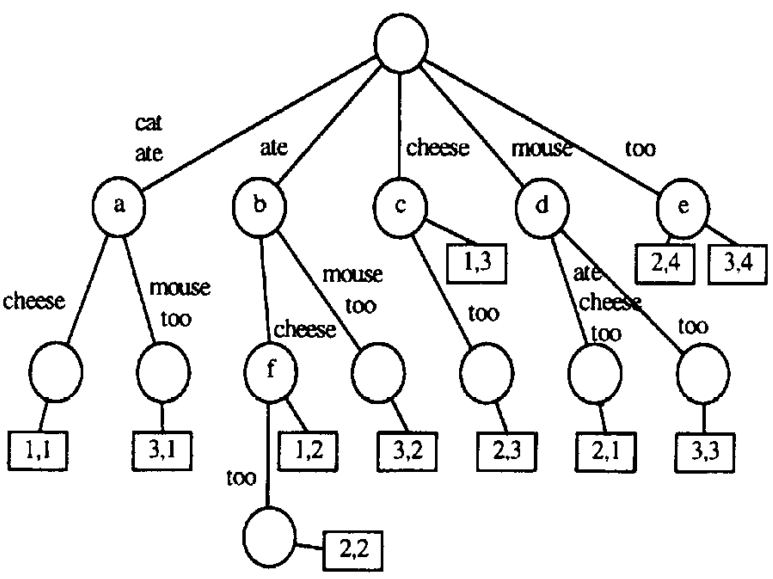
\includegraphics[totalheight=0.3\textheight]{Figures/suffixtree}
  \end{center}
  \caption{A suffix tree generated from the strings “cat ate cheese”, “mouse ate cheese too” and “cat ate mouse too”. From \citetitle{Oren1998} \protect \parencite[p. 48]{Oren1998}}
  \label{fig:suffixtree}
\end{figure}

Each internal node is a phrase cluster made up of all the documents that share that phrase (i.e the union of the documents in it's descendant nodes). Each node makes up a base cluster \cite{Oren1998}. The base clusters are scored according to the scoring function: 
%Math formula
\begin{displaymath}s(B) = 
\vert B \vert \cdot f(\vert P \vert)
\end{displaymath} 
where \(\vert B \vert\) 
is the number of documents in the cluster \(B\) and  \(f(\vert P \vert)\) is a function on the length of the cluster phrase \(P\) (excluding stop words) which penalizes short phrases (\( \vert P \vert < 2\)), gives a linear score for regular phrases (\(\vert P \vert = {2,\dots,6}\)) and a constant score to longer phrases (\( \vert P \vert > 6\)). Clusters with many documents and/or long phrases receive higher scores than clusters with few documents and/or short phrases. A promising parameter identified in this step would be the score-threshold used by the \(f(\vert P \vert)\)-function. The scoring-threshold determines which of the terms in a phrase that contributes to that phrase's length.If a term is contained within 3 or less documents or more than 40\% of the documents in the collection, then the term receives a score of zero and does not contribute to the phrase's length. This could influence the scores of base clusters as some base clusters could become longer or shorter. The base cluster score is used to sort the base clusters for the final step in the \STC algorithm.

\subsubsection{Base Cluster Merging}
Base cluster merging is the final step in the \STC and is an improvement of the original algorithm. \citeauthor{Oren1998} note that,
\begin{quote}
Documents may share more than one phrase. As a result, the document sets of distinct base clusters may overlap and may even be identical. To avoid the proliferation of nearly identical clusters, the third step of the algorithm merges base clusters with a high overlap in their document sets [\dots] \cite[][3]{Oren1998}
\end{quote}
Clusters are merged based on their similarity. \citeauthor{Oren1998} use the Jaccard Similarity Coefficient which is defined as 
\begin{math}
\frac{\vert X \cap Y \vert} {\vert X \cup Y \vert}
\end{math},
where the similarity can vary between zero if there are no common elements in set \(X\) and \(Y\) and one if the two sets have all elements in common \cite{VanRijsbergen1979}.

Given two base clusters \(B_(m)\) and \(B_(n)\) and the formula for the Jaccard Similarity Coefficient the similarity between the two clusters can be calculated with:

\begin{displaymath} 
J_{m}(B_{m},B_{n}) = 
\frac{\vert B_{m} \cap B_{n} \vert} {\vert B_{m} \vert}
\end{displaymath}

\begin{displaymath} 
J_{n}(B_{m},B_{n}) = 
\frac{\vert B_{m} \cap B_{n} \vert} {\vert B_{n} \vert}
\end{displaymath}

Iff \(J_{m} > 0.5\) and \(J_{n} > 0.5 \) then the similarity of the two clusters \(m\) and \(n\) is equal to one. All base cluster pairs with a similarity of 1 is connected in a base cluster graph. This results in a set of connected components in the graph. Each connected component is considered a cluster in the final clustering result. In this last step two parameters can be identified. One could adjust the number of base clusters used to create the final clusters. The lowest scoring base clusters might not be relevant for the final results as the documents in these clusters share few of their phrases with each-other. On the other hand it might hurt the results if the algorithm use too few of the base clusters resulting in a lower number of merged clusters, or even less accurate merged clusters.

It is also possible to adjust the similarity threshold used by the Jaccard coefficient, or use another similarity measure all together. One such similarity measure is the cosine similarity measure that can be used when documents are represented in a vector space model. This similarity measure is used by \cite{Chim2007}, albeit with phrases in a hierarchical clustering algorithm. The cosine similarity formula returns a value between -1 and 1, where -1 denotes that the vectors being compared are completely dissimilar, 1 that they are identical, and 0 that they are somewhere in between. The cosine similarity value can easily be applied as a similarity measure when combining clusters.

\subsection{Compact Trie Clustering}
The \CTC algorithm is a slightly modified version of the \STC algorithm, developed by \supervisor. The algorithm is so named because it use k-grams instead of suffixes, and because it also follows the compact tree structure. A k-gram is a subsequence of \(k\) number of characters occurring in a sequence of characters (a word or term). In the word ``mouse'' all the 3-grams would be 
\begin{inparaenum}[(1)] 
    \item mou
    \item ous
    \item use
\end{inparaenum}
(ignoring start and end \$-signs)
\cite{Manning2009}. A k-gram can also be applied on sentences. the k-grams of a sentence is all the subsequences of \(k\) words occurring in that sentence. The 3-grams of the sequence ``mouse ate cheese too'' is
\begin{inparaenum}[(1)] 
    \item mouse ate cheese
    \item ate cheese too
\end{inparaenum}.
Tests performed by the LLI research group indicate that using k-grams in the expansion phase may yield better time performance when compared with suffix expansion. Because speed is one of the requirements set by \cite{Oren1998} for web document clustering it is interesting to investigate the use of k-grams for snippet expansion.

\subsection{Performance measures}
What kind of performance measures are used for clustering...

\subsection{Available corpora}
Which corpora are used in clustering and/or classification research? Which ones are suited to clustering? Which ones are used in this master thesis research? Explain scope...


\section{Genetic Algorithms}
\label{GeneticAlgorithm}
General overview of a genetic algorithm here.


\section{Related Work}
\label{RelatedWork}
Introduce related research work in this chapter.